\documentclass[a4paper,12pt]{article}
\usepackage{extsizes}
\usepackage[english, russian]{babel}
\usepackage[pdftex]{graphicx}
\usepackage[T2A, T1]{fontenc}
\usepackage[utf8]{inputenc}
\usepackage{caption}
\usepackage{amsthm}
\usepackage{amsmath}
\usepackage{amsfonts}
\usepackage{geometry}  % установка полей
\usepackage{cases}
\geometry{top=3.5cm,bottom=2cm,left=2cm,right=2cm}
%\usepackage{graphicx}
\graphicspath{}
\DeclareGraphicsExtensions{.pdf,.png,.jpg,}
%\renewcommand{\figurename}{Рис}
\renewcommand{\figurename}{Рис.}
\renewcommand{\d}{\displaystyle}
%\renewcommand{\rmdefault}{ftm}
\newtheorem*{note}{Замечание} \theoremstyle{remark}
\newtheorem*{theorems}{Теорема}
\newtheorem*{conjecture}{Гипотеза}
\begin{document}

\begin{titlepage}
\newpage

\begin{center}
\vspace{1.5cm}
Московский государственный университет \\*
имени М.В.~Ломоносова \\*
\hrulefill
\end{center}

\flushright{\large Курсовая работа}

\vspace{7em}

\begin{center}
\Large Одномерные течения суспензии в пористой среде с учётом отложения частиц 
\end{center}

\vspace{1em}

\begin{center}
\Large One-dimensional flows of suspension with consideration of particle deposition
\end{center}

\vspace{2.5em}

\begin{center}
\textsc{\textbf{Механико-математический факультет МГУ \linebreak Кафедра гидромеханики}}
\end{center}

\vspace{3.5em}

\begin{flushright}
Научный руководитель:
\end{flushright}

\begin{flushright}
\large \textit{Н.Е.~Леонтьев}
\end{flushright}

\begin{flushright}
Работу выполнил:
\end{flushright}

\begin{flushright}
студент группы \textbf{524}\\
\vspace{1em}
\large \textit{Андрей Волчанский}\\
\end{flushright}

\vspace{\fill}

\begin{center}
Москва 2017
\end{center}

\end{titlepage}

\tableofcontents
\pagebreak


\section{Введение}

\par В большинстве природных процессов фильтрация жидкости сквозь пористую среду происходит в условиях наличия в жидкости мелких в масштабах течения частиц. Примерами таких течений могут быть течение загрязнённой воды сквозь очищающий слой фильтра, закачка пропанта в трещину в задаче о гидроразрыве.
\par Характерными особенностями таких задач являются движение маленьких частиц в относительно высоких концентрациях, которое происходит со скоростями, равными скорости несущего флюида и загрязнение фильтрующего пласта, которое сопровождается изменением пористости и других параметров. В данной работе была рассмотрена одномерная модель загрязнения пласта, где загрязнение моделируется кинетическим уравнением, отложение частиц зависит от скорости жидкости, пористости и концентрации частиц, а также были получены решения для функций пористости и концентрации частиц.

\pagebreak

\section{Основные уравнения}

\subsection{Определения теории фильтрации}

\par Вспомним некоторые элементы теории фильтрации  и добавим новое понятие --- осаждение.\\
\par Осаждение --- процесс прилипания мелких частиц, содержащихся в фильтруемой жидкости, к скелету пористой среды.\\
\par Пусть $\alpha(x^{i},t)$ --- объёмная концентрация взвешенных частиц, $m(x^{i},t)$ --- пористость, то есть отношение объёма пор к объёму малого участка среды.\\
\begin{figure}[h!]
\center{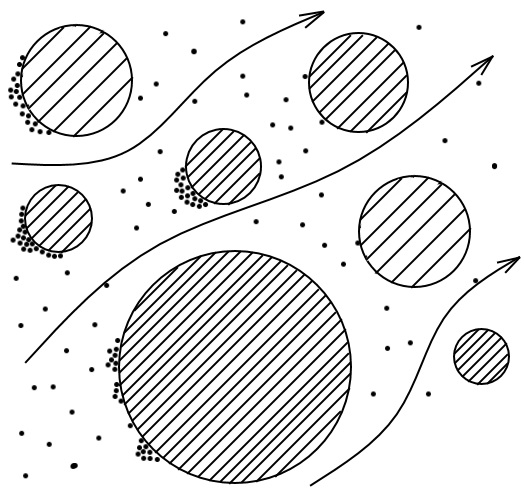
\includegraphics[width=7cm]{Particles_and_skeleton.jpg}}
\caption{Схема течения на уровне пор}
\label{fig:image1}
\end{figure}
\begin{conjecture}
Частицы имеют размер много меньше размера пор (во многих приложениях размер пор $d_{\text{ч}}\approx$ 1 мкм), перемещаются только благодаря потоку жидкости, перемешивание отсутствует. Значит, скорость частиц равна скорости жидкости. Предполагается, что жидкость и частицы --- \textit{несжимаемые}. $\rho_{\text{ч}} = const, \; \rho_{\text{жидк}}\equiv\rho = const$
\end{conjecture}

\begin{figure}[h!]
\center{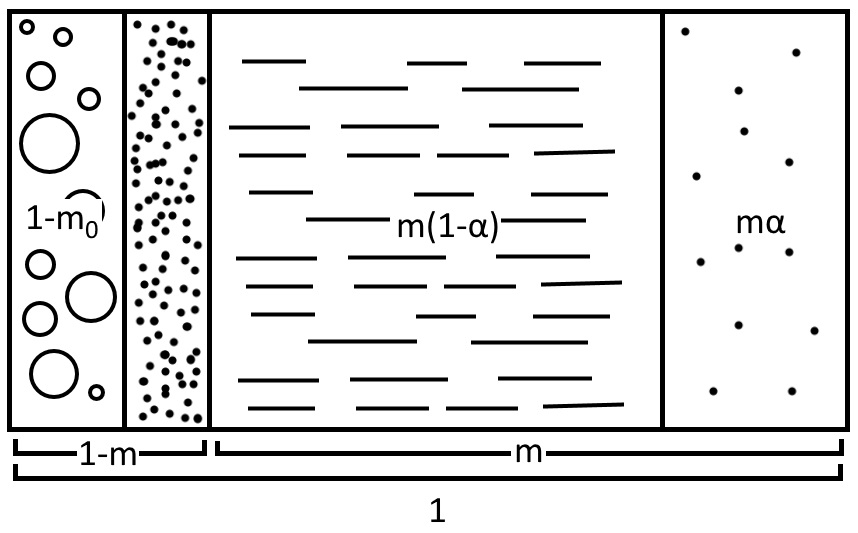
\includegraphics[width=10cm]{particles_quantity.jpg}}
\caption{Количество частиц в терминах $\alpha$ и $m$}
\label{fig:image2}
\end{figure}


\subsection{Законы сохранения массы}
\par Как и в других разделах механики сплошной среды, в теории фильтрации действуют стандартные законы сохранения. Их можно записать для каждой из фаз, для флюида и для частиц.
\par Запишем закон сохранения массы для жидкости:
$$\displaystyle \frac{d}{dt}\int\limits_{V}\rho m (1-\alpha)\,dV = - \int\limits_{\Sigma}\rho u_{n}(1-\alpha)\,d\sigma$$

\par Применяя стандартеную технику перехода к дифференциальной форме, получим уравнение неразрывности для жидкой фракции:
$$
\begin{aligned}
\displaystyle 
\frac{\partial}{\partial t}(m(1-\alpha))+div((1-\alpha)\vec{u})=0
\end{aligned}
\eqno{(1)} 
$$
\par Также можно выписать соотношение на разрыве: 
$$[m(1-\alpha)]D-[(1-\alpha)u_{n}]=0$$
\par или в эквивалентной форме:
$$[m(\alpha-1)]D-[\alpha u_{n}]=0$$

\par Запишем аналогичный закон для частиц.

$$\displaystyle \frac{d}{dt}\int\limits_{V}{\rho_{\text{ч}}m\alpha+\rho_{\text{ч}}((1-m)-1-m_{0})}dV=-\int\limits_{\Sigma}\rho_{\text{ч}}\vec{u}\alpha d\sigma$$
\par Здесь $m_{0}=const$ --- первоначально однородный пласт. Перепишем полученные равенства в виде уравнения неразрывности:\\
$$(m\alpha)_{t}-m_{t}+div(\alpha \vec{u})=0$$
$$
\begin{aligned}
\displaystyle 
(m\alpha)_{t}+div(\alpha \vec{u})=m_{t}
\end{aligned}
\eqno{(2)} 
$$

\par Соотношение на разырыве:
$$[m\alpha-m]D-[\alpha u_{n}]=0$$

\par \textbf{Следствие:} Складывая (1)+(2) получаем уравнение неразрывности для \textbf{всей} суспензии.\\
$$m_{t}+div\;\vec{u}=m_{t}$$
$$div\;\vec{u}=0$$
\par Это уравнение можно использовать вместо (1) или (2) при решении системы уравнений.

\subsection{Закон Дарси}
\par В теории фильтрации используется экспериментальный закон Дарси, который связывает скорость и градиент давления. Этот закон можно получить как частное следствие закона Навье-Стокса при осреднении. Закон Дарси имеет вид:
$$
\begin{aligned}
\displaystyle 
-\vec{\nabla}P-\frac{\mu}{k}\vec{u}=0
\end{aligned}
\eqno{(3)} 
$$
\par В нашей постановке полагается, что массовых сил нет. Приведём известные зависимости для вязкости:
$\mu=\mu(\alpha)=\mu_{0}(1+C\alpha)\approx\mu_{0},\;\;$
$k=k(m)$
\par Обычно (3) отщепляется от системы.

\subsection{Кинетическое уравнение}

\par В исследуемой задаче функция, описывающая отложение частиц, считается известной, мы будем полагать, что данная зависимость имеет следующий вид:
$$
\begin{aligned}
\displaystyle 
m_{t}=-f(|\vec{u}|, m,|\vec{\nabla} P| , \alpha)
\end{aligned}
\eqno{(4)} 
$$

\par С учётом кинетического уравнения мы можем выписать полную систему уравнений для поставленной задачи.

$$\displaystyle \begin {cases}
(m\alpha)'_{t}+(\alpha u)'_{x}=m'_{t}\\
u'_{x}=0\\
\displaystyle -P'_{x}-\frac{\mu}{k}u=0\\
m_{t}=-f(|\vec{u}|, m,|\vec{\nabla} P| , \alpha)\\
\end {cases}$$

\subsection{Классификация системы уравнений}
\par В системе 6 уравнений и 6 неизвестных, $m, \alpha, P, \vec{u}$\\
\par Выписав систему уравнений для одномерных течений, можно получить матрицы с коэффициентами при производных переменных по $t$ (матрица $A_{ij}$) и по $x$ ($a_{ij}$). Если при этом у характеристического уравнения $|A_{ij}x-a_{ij}|=0$ все корни действительные, то система гиперболическая. Иначе говоря, если уравнения отделятся друг от друга в смысле производных неизвестной величины. Для нашей системы:\\
\bigskip
\\
$
\begin{cases}
\begin{aligned}
&(m\alpha)'_{t}+(\alpha u_{0})'_{x}=m'_{t}\\
&m_{t}=-f(|\vec{u}|, m,|\vec{\nabla} P| , \alpha)
\end{aligned}
\end{cases}$
$\Leftrightarrow$
$
\begin{cases}
\begin{aligned}
&m\alpha'_{t}+\alpha m'_{t}+u_{0}\alpha'_{x}=m'_{t}\\
&m_{t}=-f(|\vec{u}|, m,|\vec{\nabla} P| , \alpha)
\end{aligned}
\end{cases}$\\
\medskip
$\\
\begin{cases}
\begin{aligned}
&m\alpha'_{t}+(\alpha-1) m'_{t}+u_{0}\alpha'_{x}=0\\
&m_{t}=-f(|\vec{u}|, m,|\vec{\nabla} P| , \alpha)
\end{aligned}
\end{cases}$
$\Leftrightarrow$
$
\begin{cases}
\begin{aligned}
&m\alpha'_{t}+u_{0}\alpha'_{x}=(\alpha-1)f(|\vec{u}|, m,|\vec{\nabla} P| , \alpha)\\
&m_{t}=-f(|\vec{u}|, m,|\vec{\nabla} P| , \alpha)
\end{aligned}
\end{cases}$\\
\bigskip
\\
\par Можно разделить производные (в каждом уравнении производные вдоль своего направления), значит система гиперболическая.
\pagebreak
\section{Постановка задачи}
\subsection{Одномерное течение}
\par В этой работе рассматривается одномерное течение жидкости с частицами сквозь пористую среду. Выпишем систему уравнений для одномерного течения:
$$\displaystyle \begin {cases}
(m\alpha)'_{t}+(\alpha u)'_{x}=m'_{t}\\
u'_{x}=0\\
\displaystyle -P'_{x}-\frac{\mu}{k}u=0\\
m_{t}=-f(|\vec{u}|, m,|\vec{\nabla} P| , \alpha)\\
\end {cases}$$

\par Сделаем следующие предположения. Пусть скорость $u=q(t)$ --- функция времени t, а так же $q=q_{0}=const(=u_{0})$. Получили следующую систему:\\
$$\begin {cases}
(m\alpha)_{t}+\alpha_{x}u_{0}=m_{t}\\
m_{t}=-f(|\vec{u}|, m,|\vec{\nabla} P| , \alpha)
\end{cases}$$
\par Получившаяся в результате предположений система является квазилинейной и содержит две неизвестные.

\subsection{Граничные условия}
\par В задаче рассматриваются следующие граничные условия:
\par \textbf{На входе} в пласт положим заданной концентрацию частиц $\alpha|_{x=0}=\alpha_{0}(t)$ и, в частности, $=const$\\
\par В начальный момент времени $t=0$ считаем заданной пористость среды  $m=m_{0},\text{а концентрацию}\;\;\alpha=0$ --- внутри пористой среды первоначально \textbf{чистая} жидкость.\\
\par \textbf{На выходе} из пласта при $x=L$ условия не ставятся, что связано с поведением характеристик.\\
\pagebreak
\subsection{Начало закачки в пласт}
\par Приведём иллюстрацию процесса для переменных $m$ и $\alpha$ соответственно:
\begin{figure}[h!]
\center{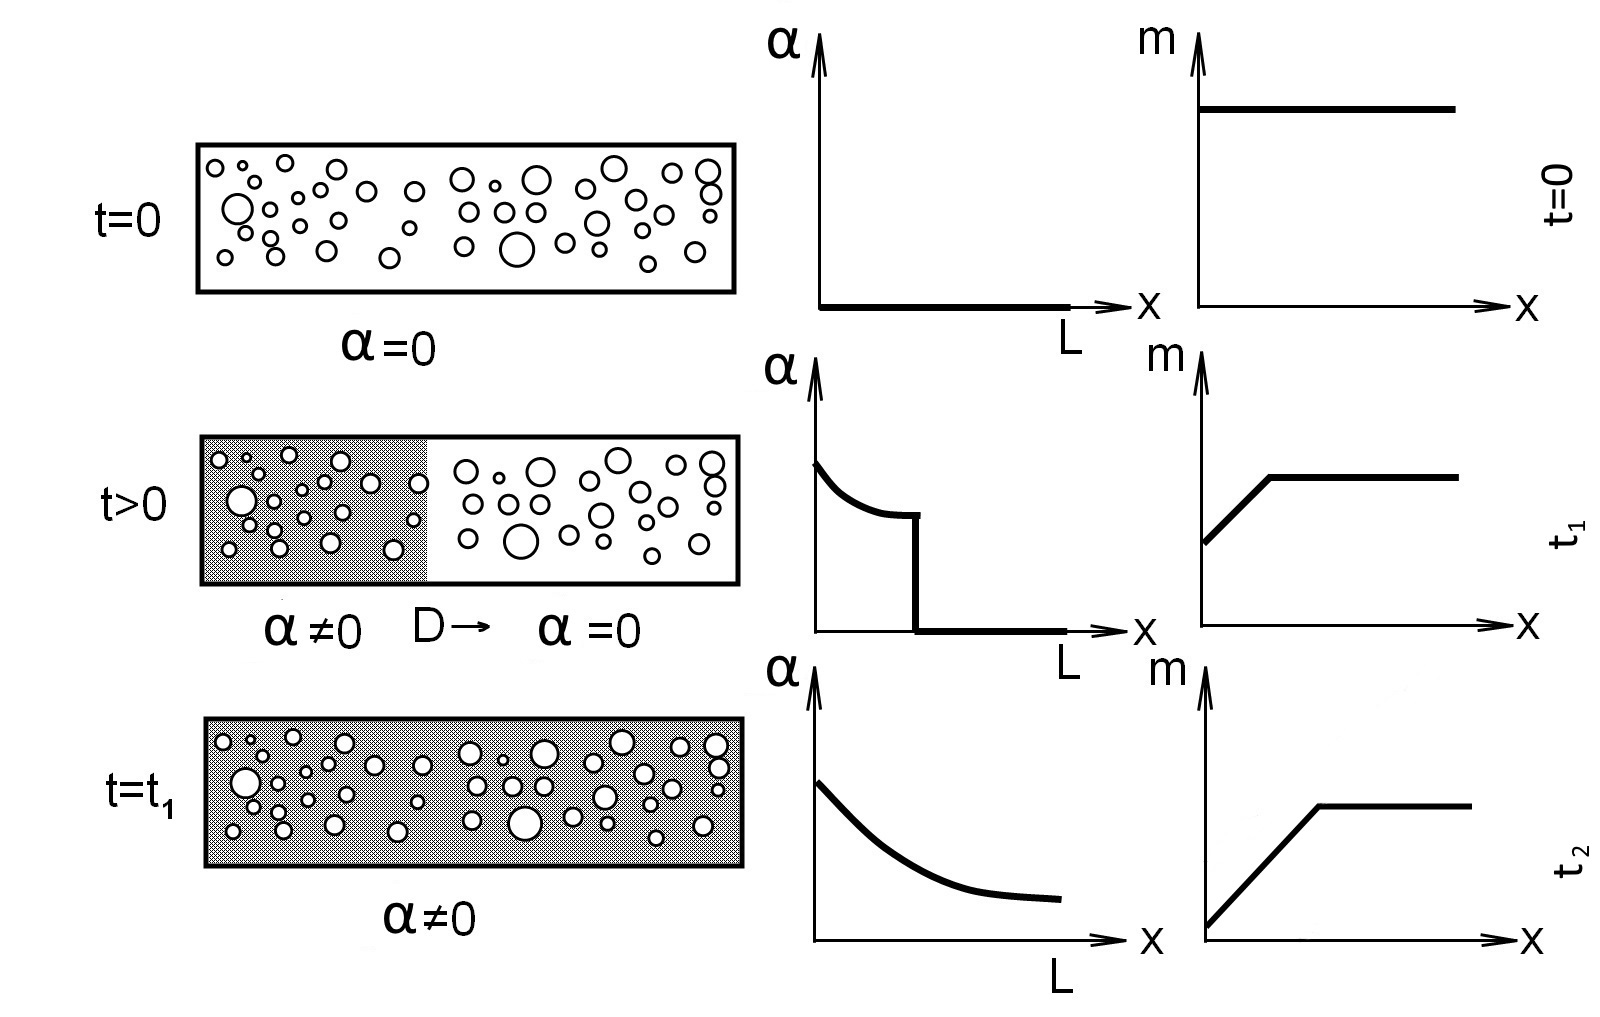
\includegraphics[width=15cm]{begining_of_loading.jpg}}
\caption{}
\label{fig:image1}
\end{figure}
\pagebreak
\section{Решение упрощённой задачи с конкретным уравнением засорения}
\subsection{Дополнительные предположения}
\par Предположим, что $m\approx m_{0}$, то есть изменение пористости можно считать малым. Также можно предположить $\alpha\ll 1$ --- концентрация мала. Тогда от уравнения $$m_{t}\alpha + m\alpha+u_{0}\alpha_{x}=m_{t}$$ можно перейти к $$m_{0}\alpha_{t}+u_{0}\alpha_{x}=m_{t}$$ Добавим в систему частный случай кинетического уравнения засорения: $m_{t}=-\gamma \alpha |u_{0}|$, где множитель $\alpha |u_{0}|$ пропорционален объёму жидкости, протекающей через данную точку, а $\gamma=const$ --- экспериментальный коэффициент, который, например, в общем случае может зависеть от пористости. Далее мы проверим, что есть решение $\alpha=\alpha(x)$ за фронтом (не зависит от $t$, однако $m$ от времени зависит).\\
\par В итоге получаем уравнение $$\alpha'_{t}+\frac{u_{0}}{m_{0}}\alpha'_{x}=-\frac{\gamma\alpha |u_{0}|}{m_{0}}$$ 
\par Уравнению засорения соответствует характеристика $\d \frac{dx}{dt}=const$, а уравнению выше --- $\d\frac{dx}{dt}=\frac{u_{0}}{m_{0}}$. Поскольку разрыв идёт вдоль второй характеристики, то от разрыва уходит только одна характеристика --- закон сохранения массы выполняется. Выпишем соотношение на разрыве: $[m(1-\alpha)]D-[(1-\alpha)u_{n}]=0,$ где $u_{n}=u_{0}$. Тогда: $m_{0}[1-\alpha]\frac{u_{0}}{m_{0}}-[1-\alpha]u_{0}=0$. Здесь мы пользуемся гипотезой $[m]=0$, но возможны и другие ситуации. \\
\par Итак, можно поставить следующую задачу: при заданной $\alpha|_{x=0}=\alpha_{0}$ найти решение $\alpha(x)$ за скачком, а также $m=m(x,t)$. 
\subsection{Решение поставленной задачи}
\par Найдём решение уравнения вдоль характеристики $\d \frac{dx}{dt}=0$: $$\d \alpha_{t}+\frac{u_{0}}{m_{0}}\alpha_{x}=-\frac{\gamma\alpha|u_{0}|}{m_{0}}$$ 
\par Отсюда получаем $\d \frac{d\alpha}{dt}=-\frac{\gamma\alpha|u_{0}|}{m_{0}}$. $\d \int\frac{d\alpha}{\alpha}=-\int\frac{\gamma|u_{0}|}{m_{0}}dt$, откуда окончательно получаем $$\d ln\;\alpha=-\frac{\gamma|u_{0}|}{m_{0}}t+C$$\\
\par Перепишем полученное решение в виде $\d ln\frac{\alpha}{\alpha_{0}}=-\frac{\gamma|u_{0}|}{m_{0}}(t-t_{0})$. Так же, вспоминая, что мы искали решение вдоль характеристики, из $\d \frac{dx}{dt}=\frac{u_{0}}{m_{0}}$ можем получить $\d x=\frac{u_{0}}{m_{0}}(t-t_{0})$. Это показывает, что найденное решение можно представить в виде $\alpha=\alpha_{0}e^{-\gamma x}$, или 
\begin{equation*}
\d
\alpha=
\begin{cases}
\d
\alpha_{0}e^{-\gamma x},\;\;& x<\frac{u_{0}}{m_{0}}t\\
0,\;\;& x\geq \frac{u_{0}}{m_{0}}t\\
\end{cases}
\end{equation*}
 Представляя это решение как $\d \alpha=\alpha_{0}e^{-\gamma \frac{u_{0}}{m_{0}}(t-t_{0})}$, можно получить, что скорость разрыва $\d D=\frac{u_{0}}{m_{0}}$. Проверим выпонение условия баланса массы на скачке: $[m(1-\alpha)]D-[(1-\alpha)u_{n}]=0$, откуда $m_{0}[1-\alpha]D-[1-\alpha]u_{n}=0$. Так как $m_{0}D-u_{n}=0$, то отсюда следует $u=u_{0}=const$\\
\par Размерность величины $\gamma$ имеет вид $[\gamma]=\textbf{1/м}$. Её можно трактовать как типичную длину засорения, так как величина $\alpha/\alpha_{0}$ падает в $e$ на расстоянии $1/\gamma$ от начала координат.\\
\par Также у нас осталось уравнение $m_{t}=-\gamma u_{0}\alpha$. С его помощью найдём решение 
\begin{equation*}
\d
m=m|_{t=0}+\int\limits^{t}_{0}m_{t}dt=m_{0}-\int\limits^{t}_{0}\gamma u_{0}\alpha dt=
\begin{cases}
\d
m_{0}-\gamma u_{0}\alpha(x)(t-\frac{xm_{0}}{u_{0}}),\;\;& x<\frac{u_{0}}{m_{0}}t\\
m_{0},\;\;& x\geq \frac{u_{0}}{m_{0}}t\\
\end{cases}
\end{equation*}
\pagebreak
\section{Решение задачи без упрощений}
\subsection{Полное уравнение.}
\par Теперь получим решение в случае, когда $m=m(x,t)$ Имеем систему 
\begin{equation*}
\begin{cases}
(m\alpha)_{t}+u_{0}\alpha_{x}&= m_{t}\\
m_{t}&= -\gamma u_{0}\alpha\\
\end{cases}
\end{equation*}
\par Подставляя второе в первое и раскрывая скобки, получим $$\d \alpha_{t}+\frac{u_{0}}{m}\alpha_{x}=(\alpha-1)\gamma\frac{u_{0}}{m}\alpha$$
\par Рассматривая характеристики $\d \frac{dx}{dt}=\frac{u_{0}}{m}$ и интегрируя соотношение, получаем $\d \int \frac{d\alpha}{\alpha^{2}-\alpha}=\int\gamma dx=\int\frac{d(\alpha-1)}{\alpha-1}-\int\frac{d\alpha}{\alpha}$. Интегрируя и потенцируя, получаем окончательно выражение для $\alpha$:
\begin{equation*}
\d
\alpha=
\begin{cases}
\d
\frac{1}{1-\frac{\alpha_{0}-1}{\alpha_{0}}e^{\gamma x}},\;\;& x<\frac{u_{0}}{m}t\\
0,\;\;& x\geq \frac{u_{0}}{m}t\\
\end{cases}
\end{equation*}

\par Теперь, зная решение для $\alpha$, можно выразить $m$: $ \d
m= m|_{t=0}+\int\limits^{t}_{0}m_{t}dt=m_{0}+\int\limits^{t}_{0}\gamma u_{0}\alpha=m_{0}+\int\limits^{t}_{\frac{xm_{0}}{u_{0}}}\gamma u_{0}\frac{1}{1-\frac{\alpha_{0}-1}{\alpha_{0}}e^{\gamma x}} dt=$
\begin{equation*}
=
\begin{cases}
\d
m_{0}-\gamma u_{0}\frac{1}{1-\frac{\alpha_{0}-1}{\alpha_{0}}e^{\gamma x}}=(t-\frac{xm_{0}}{u_{0}}),\;\;& x<\frac{u_{0}}{m_{0}}t\\
m_{0},\;\;& x\geq \frac{u_{0}}{m_{0}}t\\
\end{cases}
\end{equation*}

\par Можно заметить, что полученное решение при $\alpha_{0} \rightarrow 0$ переходит в полученное ранее выражение $$\d \alpha=\frac{1}{1-\frac{\alpha_{0}-1}{\alpha_{0}}e^{\gamma x}}\approx\frac{\alpha_{0}}{e^{\gamma x}}$$
\pagebreak

\section{Решения в виде рядов}
%\subsection{Различия с решённой задачей}
\par Существует метод поиска точных решений путём разложения общего уравнения в ряд по концентрации осаждённых частиц. Если полагать, что скорость отложения частиц не просто пропорциональна  модулю скорости фильтрации, а есть некоторая функция пористости, то система переписывается следующим образом.

\par Обозначим концентрацию осаждённых частиц $s = (1-m_{0})-(1-m)$. Тогда нашу систему можно записать как:

\begin{equation*}
\begin{cases}
(a(s)\alpha+s)_{t}+(b(s)\alpha)_{x}&= 0\\
-(s)_{t}&=K(s)\alpha\\
\end{cases}
\end{equation*}

\par Сопоставим коэффициенты, зависящие от $s$ с обозначениями в решённых задачах. $a(s)$ --- $m$, $b(s)$ --- $u_{0}$, $K(s)$ --- $-\gamma u_{0}$. Полученные этим способом функции $s$ и $\alpha$ расширяют класс решений, полученных в рассмотренных предельных случаях. 

\par Полагая $K(s)=\varepsilon\Lambda(s)$, где $\varepsilon$ --- малый параметр и раскаладывая функции $a(s)$, $b(s)$ и $\Lambda(s)$ в ряды по $s$ в окрестности нуля. Это справедливо, так как всё ещё принята гипотеза о слабом засорении. Таким образом получим системы дифференциальных уравнений на коэффициенты рядов, решая которые можно получить решения необходимой точности в данном классе решений.
\par Решения ищутся в виде $s(x,t,\varepsilon)=\varepsilon s_{1}(x,t)+\varepsilon^{2} s_{2}(x,t)+...$
\par Выпишем эти системы для нескольких членов разложения:

\begin{equation*}
\varepsilon^{1}: 
\begin{cases}
(a_{0}\alpha_{1}+a_{1}\alpha_{0}s_{1})_{t}+(b_{0}\alpha_{1}+b_{1}\alpha_{0} s_{1})_{x}&= -\lambda_{0} \alpha_{0}\\
-(s_{1})_{t}&= - \lambda_{0} \alpha_{0}\\
\end{cases}
\end{equation*}

\begin{equation*}
\varepsilon^{2}: 
\begin{cases}
(a_{0}\alpha_{2}+a_{1}\alpha_{1}s_{1}+a_{2}\alpha_{0} s_{1}^{2}+a_{1}\alpha_{0}s_{2})_{t}+\\+(b_{0}\alpha_{2}+b_{1}\alpha_{1} s_{1}+b_{2}\alpha_{0}s_{1}^{2}+b_{1}\alpha_{0} s_{2})_{x}&= -(\lambda_{0} \alpha_{1}+\lambda_{1}\alpha_{0}s_{1})\\
-(s_{2})_{t}&= - (\lambda_{0} \alpha_{1}+\lambda_{1}\alpha_{0}s_{1})\\
\end{cases}
\end{equation*}

\par Решая последовательно эти системы методом характеристик можно получить искомое решение с необходимой наперёд заданной точностью.

\pagebreak

\section{Расширенный класс решений}
\subsection{Система уравнений для обобщённого кинетического уравнения}
\par Ранее рассмотренное кинетическое уравнение имело довольно простой вид, а именно $m_{t} = -u_{0}\gamma \alpha$, теперь мы попробуем придать ему более общий вид. Как отмечалось ранее, функция, характеризующая изменение пористости со временем зависит от пористости в текущий момент времени. Пусть теперь кинетическое уравнение имеет вид $m_{t} = -F(m)\alpha$, где $F(m)$ --- произвольная функция. Перепишем нашу систему уравнеий:
\begin{equation*}
\begin{cases}

(m\alpha)_{t}+ u_{0}\alpha_{x} &= m_{t}\\
m_{t} &= -F(m)\alpha\\

\end{cases}
\end{equation*}

\par В отличие от рассмотренных до этого задач, мы перейдём не к переменной $\alpha$, а к переменной $m$. Пусть $\d G(m) = -\frac{1}{F(m)}$. Тогда
$$\Big(m \big(G(m)m_{t} - 1\big)\Big)_{t} + u_{0}\big(G(m)m_{t}\big)_{x} = 0$$

\par Докажем, что $\big(G m_{t}\big)_{x} = \big(G m_{x}\big)_{t}$.\\
$\d \big(G(m)m_{t}\big)_{x} = G_{m}m_{t}m_{x} + G m_{tx} = \big(G m_{x}\big)_{t}$, откуда следует, что в нашем уравнении можно поменять местами производные по времени и по координате, а именно, получим:
$$\Big(m \big(G(m)m_{t} - 1\big)\Big)_{t} + u_{0}\big(G(m)m_{x}\big)_{t} = 0$$
\par Данное уравнение можно проинтегрировать по времени. Получим следующее:\\
$$m \big(G(m)m_{t} - 1\big) + u_{0}G(m)m_{x} = \Phi(x)$$
где $\Phi(x)$ --- произвольная функция.
\par Переписывая последнее уравнение, получим:
$$m_{t}+\frac{u_{0}}{m}m_{x}=\frac{m+\Phi(x)}{G(m)m}$$
\par Это уравнение гиперболическое. Решая его методом характеристик можем получить выражение для пористости.\\
\begin{equation*}
\begin{cases}

\d \frac{dm}{dt} &= \d \frac{m+\Phi(x)}{G(m)m}\\
&\\
\d \frac{dx}{dt}&= \d \frac{u_{0}}{m}\\
&\\
m_{t} &= -F(m)\alpha\\

\end{cases}
\end{equation*}

\par Решением одной из упрощённых задач было выражение на $m$:\\
$$m = m_{0} - \gamma u_{0}\frac{t-\frac{xm_{0}}{u_{0}}}{1 - \frac{\alpha_{0}-1}{\alpha_{0}}e^{\gamma x}}=m_{0}-\gamma u_{0}\theta$$
\par Найдём такую функцию $\Phi(x)$, которая соответствует данному решению. $G(m)=-\frac{1}{\gamma u_{0}}$. Для удобства выпишем, чему равны производные этого решения:\\
$$m = m_{0} - \gamma u_{0}\theta(t-\frac{xm_{0}}{u_{0}})$$
$$m_{t} = -\gamma u_{0}\theta$$
$$m_{x} = \gamma u_{0}\theta\frac{m_{0}}{u_{0}}-\gamma u_{0}(t-\frac{xm_{0}}{u_{0}})\theta^{2}\frac{\alpha_{0}-1}{\alpha_{0}}e^{\gamma x}\gamma$$\\
\par Подставляя и приводя подобные, получим $\Phi(x)=-m_{0}$.
\par Теперь, имея всю необходимую информацию, можно попробовать решить расширенную систему уравнений, используя новые знания о функции $\Phi(x)$.

\begin{figure}[h!]
\center{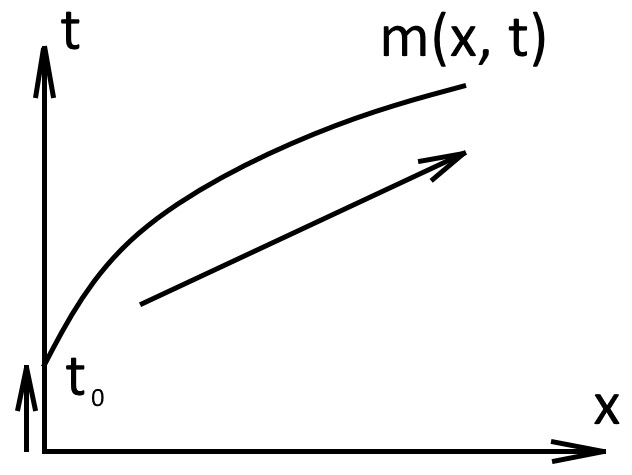
\includegraphics[width=7cm]{characteristics_solution_scheme.jpg}}
\caption{Схема решения методом характеристик.}
\label{fig:image1}
\end{figure}

\par В системе, которую мы уже писали раньше, заменим производную по времени производной по координате, что справедливо, поскольку мы находимся на характеристике.

\begin{equation*}
\begin{cases}

\d \frac{dm}{dx} &= \d \frac{m+\Phi(x)}{G(m)u_{0}}\\
&\\
\d \frac{dx}{dt}&= \d \frac{u_{0}}{m}\\
&\\
m_{t} &= -F(m)\alpha\\

\end{cases}
\end{equation*}

\par Запишем условия для нашей исходной задачи на функцию $F(x)$ и граничные и начальные условия. Отсюда получается, что $\d G(x)=-\frac{1}{\gamma u_{0}}$, при $x=0$ концентрация частиц постоянна и равна $\alpha_{0}$, в начальный момент времени полагаем всюду пористость $m=m_{0} = const$.

\begin{equation*}
\begin{cases}

\d \frac{dm}{dx} = \d -\gamma (m+\Phi(x))\\
{}\\
\d \frac{dx}{dt}= \d \frac{u_{0}}{m}\\
{}\\
m_{t} = -\gamma u_{0}\alpha\\

\end{cases}
\end{equation*}

\par Получим решение в некотором параметрическом виде. Ход решения изображён на рис. 4. Сначала мы найдём, какая пористость будет на искомой характеристике при $x=0$ в момент времени $t = \hat{t}$. Решим первое уравнение в системе:

$$\frac{dm}{dx}=\gamma(m_{0}-m)$$
$$\frac{d(m_{0}-m)}{m_{0}-m}=-\gamma dx$$
$$ln(m_{0}-m)=-\gamma x + C$$
$$m_{0}-m = e^{c}e^{-\gamma x}$$
\par Теперь выразим $e^{c}$ через $m(\hat{t})$. На границе выполняется уравнение $m_{t}=-\alpha_{0}\gamma u_{0}$. Его решение имеет вид: 
$$m(x=0,t)=-\alpha_{0}\gamma u_{0}t+m_{0}$$
\par Значит, в момент времени $\hat{t}$ мы имеем пористость на входе в пласт равную $m(x=0,\hat{t})=-\alpha_{0}\gamma u_{0}\hat{t}+m_{0}$. 
\par Используем его для нахождения произвольной постоянной:
$$m_{0}-m(x=0,\hat{t})= \alpha_{0}\gamma u_{0}\hat{t} = e^{c}$$
\par Получили выражение для $m(x,\hat{t})$:
$$m =m_{0} -\alpha_{0}\gamma u_{0}\hat{t}e^{-\gamma x}$$
\par Провести дальнейшую проверку планируется в последующей работе.

\pagebreak

\section{Заключение}
\par В ходе работы была выписана система уравнений фильтрации для задачи течения суспензии сквозь пористую среду с эффектом отложения. Былло получено два аналитических решения для системы уравнений. Было проведено знакомство с методами поика решений путём разложения в ряд, а также была выполнена проверка этого метода на аналитическом решении. Была решена задача об обобщении кинетического уравнения, были получены параметры, соответствующие аналитическому решению. Также было проведено ознакомление с методом характеристик и с его помощью получены аналитические решения.

\pagebreak

\begin{thebibliography}{99}
\bibitem{article}
Кузьмина Л.И., Осипов Ю.В.,
Асимптотика задачи фильтрации суспензии в поритой среде,
Вестник МГСУ, 2015, №1, с. 54-62
\bibitem{barenblatt}
Баренблатт Г. И., Ентов В. М., Рыжик В. М.,
Движение жидкостей и газов в природных пластах, М., 
Недра, 1984
\bibitem{Basniev}
Басниев К.С., Кочина И.Н., Максимов В.М.,
Подземная гидромеханика, М., 
Недра,1993

\end{thebibliography}

\end{document}